%
% File naacl2019.tex
%
%% Based on the style files for ACL 2018 and NAACL 2018, which were
%% Based on the style files for ACL-2015, with some improvements
%%  taken from the NAACL-2016 style
%% Based on the style files for ACL-2014, which were, in turn,
%% based on ACL-2013, ACL-2012, ACL-2011, ACL-2010, ACL-IJCNLP-2009,
%% EACL-2009, IJCNLP-2008...
%% Based on the style files for EACL 2006 by 
%%e.agirre@ehu.es or Sergi.Balari@uab.es
%% and that of ACL 08 by Joakim Nivre and Noah Smith

\documentclass[11pt,a4paper]{article}
\usepackage[hyperref]{naaclhlt2019}
\usepackage{times}
\usepackage{graphicx}
\usepackage{latexsym}

\newcommand{\ahcomment}[1]{\textcolor{blue}{[#1 -AH]}}

\usepackage{url}

%\aclfinalcopy % Uncomment this line for the final submission
%\def\aclpaperid{***} %  Enter the acl Paper ID here

%\setlength\titlebox{5cm}
% You can expand the titlebox if you need extra space
% to show all the authors. Please do not make the titlebox
% smaller than 5cm (the original size); we will check this
% in the camera-ready version and ask you to change it back.

\newcommand\BibTeX{B{\sc ib}\TeX}

\title{Extractive sentence compression under lexical and length constraints}

\author{First Author \\
  Affiliation / Address line 1 \\
  Affiliation / Address line 2 \\
  Affiliation / Address line 3 \\
  {\tt email@domain} \\\And
  Second Author \\
  Affiliation / Address line 1 \\
  Affiliation / Address line 2 \\
  Affiliation / Address line 3 \\
  {\tt email@domain} \\}

\date{}

\begin{document}
\maketitle

\begin{abstract}
Traditional approaches to extractive sentence compression seek to reduce the length of a sentence, while retaining the most ``important'' information from the source. But query-focused applications such as document search engines or exploratory search interfaces place additional lexical and length requirements on compression systems. This study examines extractive sentence compression under such constraints, using both classical ILP-based methods and modern neural network techniques. We introduce a new neural compression method which can accommodate length and lexical requirements.
\end{abstract}

\section{Introduction}
Traditional study of extractive sentence compression seeks to create short, readable compressions which retain the most ``important'' information from source sentences. But query-focused and user-facing applications impose additional requirements on the output of a compression system. Compressions must be short enough to be shown in a user interface; and (often) compressions must contain a user's query term. An example of such a compression system is shown in figure \ahcomment{TODO}.


This study examines sentence compression under strict lexical and length constraints, in which a compression must be shorter than a given character budget and must include particular words. While older compression methods based on integer linear programming could trivially accommodate length and lexical restrictions, recent work has focused on neural network techniques which do not give practitioners such control. This makes existing neural methods unsuitable for search engines, concept map browsers and new forms of exploratory textual interfaces, where length and lexical constraints are paramount. \ahcomment{Cite hearst, IR book, falke, marchioni. examples.} Systems that can sometimes recreate gold training data are simply not useful for practitioners who must include query terms in shortened sentences; or scale compressions to a desktop interface or mobile phone.

\ahcomment{sign posting}

\begin{figure}[htb!]
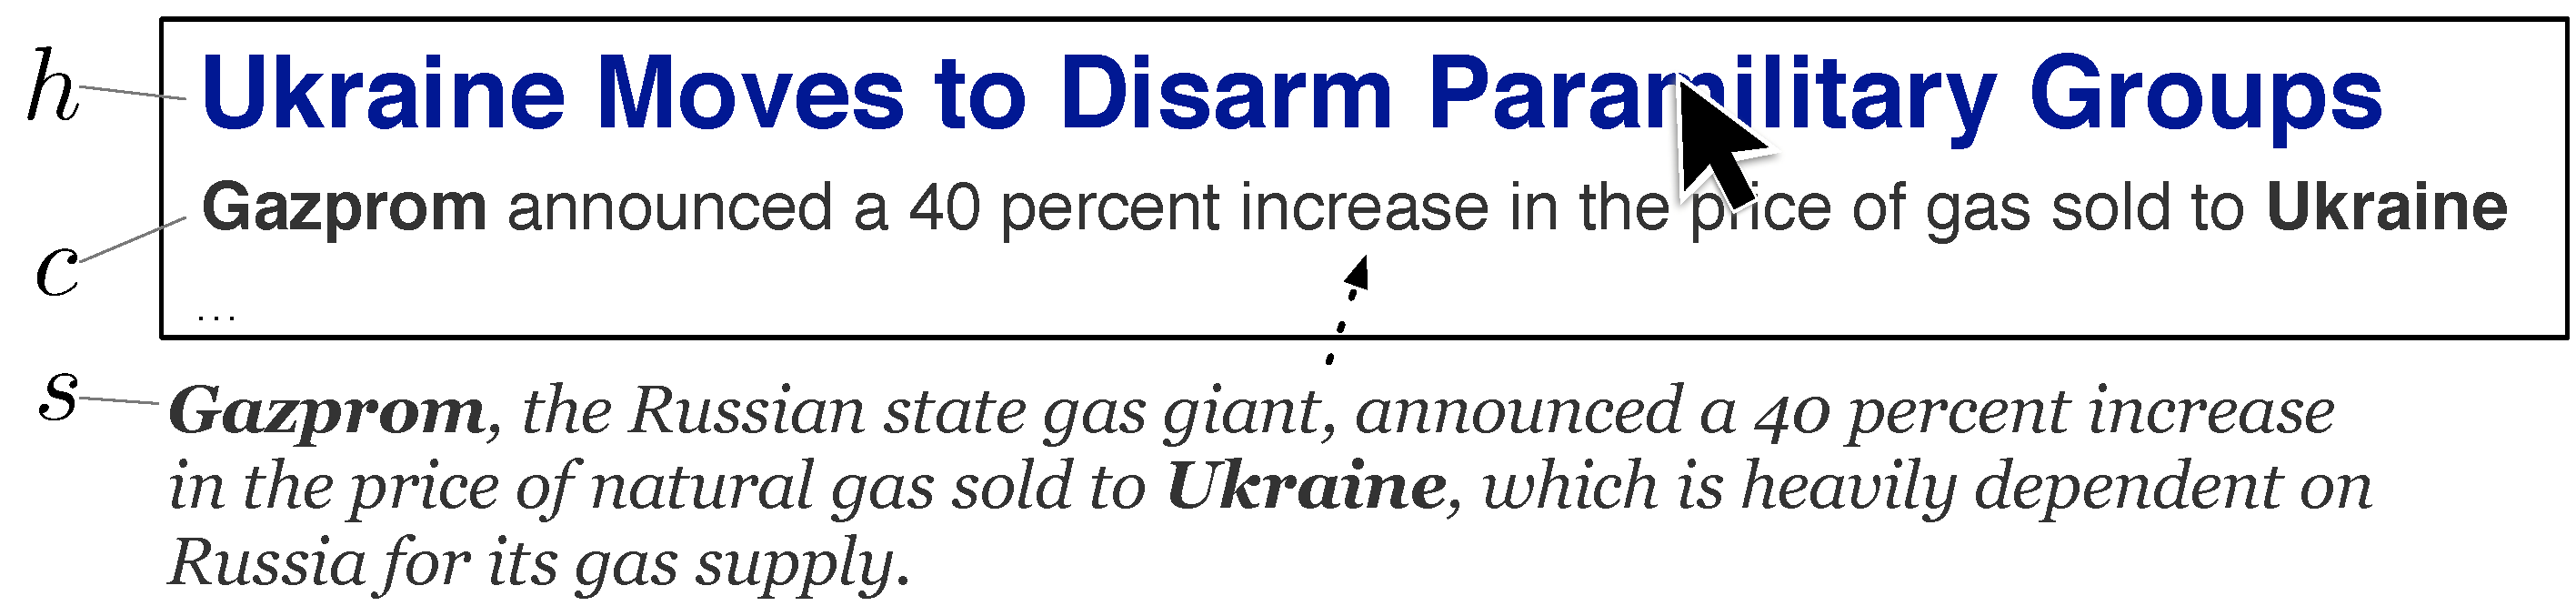
\includegraphics[width=9cm]{qf.pdf}
\caption{Search interfaces often require compressions with length and lexical constraints. In this case, the user has queried for ``Pemex contracts"; a system returns a related link and a short compression which contains the query terms}
\end{figure}


\section{Compression and constraints}

In this work, we present a new method for compressing sentences, which leverages the predictive power of neural methods while accommodating lexical and length constraints. We compare our method, \textbf{iterative deletion} to traditional \textbf{ILP-based techniques}, which also give a user such control and to baseline \textbf{LSTM taggers} which cannot accommodate such constraints.


\begin{table*}[htb!]
\begin{tabular}{cccc}
\textbf{Approach} & \textbf{Worst-case complexity} & \textbf{Constrained} & \textbf{Allows heterogenous supervision} \\ \hline
LSTM taggers      & Linear              & No     &    No      \\   
linear programming              & Exponential         & Yes    &    No   \\
iterative deletion (this work)       & Quadratic*           & Yes    &      Yes   \\
\end{tabular}
\end{table*}

\subsection{Constrained compression with ILPs}

One common approach for shortening sentences formulates compression as an integer linear programming (ILP) task. ILP-based methods assign binary variables to each token in a sentence or nested subtree in a dependency parse. These variables indicate if a word or subtree should be included in a compression. Each such sentence component is also assigned a local weight, indicating its worthiness for inclusion in a shortened sentence.\footnote{Local weights are either learned via structured perceptron techniques; or inferred from corpus statistics, tf-idf scores or language models.}

ILP methods represent the overall quality of a compression by summing the local weights of sentence components to compute a global objective score. Researchers use off-the-shelf ILP solvers to identify the highest-scoring compression, from among the exponential possible configurations of binary variables. The problem of identifying the best possible solution fo an integer programming compression objective is exponential in the number of tokens or number of subtrees in the input, as each corresponding binary variable may be set to 0 or 1.

This integer linear programming approach easily accommodates constrained compression. Often, researchers will add constraint terms to the ILP objective in order to preserve the meaning of a sentence (e.g. don't remove negations) or ensure that output forms a valid dependency tree (e.g. each subtree must have a parent vertex). Under such approaches, adding length or lexical requirements is trivial: practitioners must specify that optimal solutions must be shorter than some charascter budget and must specify that binary variables marking inclusion of particular words must be set to 1. 

\subsection{Constrained compression with pruning}

In this work, we present an alternative method for shortening sentences under lexical and length constraints. Our iterative deletion technique compresses a sentence over $M$ time steps, by pruning $M$ subtrees from a dependency parse, one after another. This method recalls early solutions to the compression problem, which also removed components of sentences. \ahcomment{CITE: K and M, Jing  and McKowen} \ahcomment{argue for coverage w/ F and A at some point}

Like ILP-based methods, iterative deletion approaches can easily accommodate lexical and length constraints: subtrees which contain query terms are never deleted, and pruning stops only when a compression satisfies a given character budget. 

However, iterative deletion methods incur much smaller computational costs than integer programming techniques. In the worst case, an iterative deletion method will prune one singleton subtree (consisting of only one vertex) at each of the $M$ timesteps during compression. (Starting from the leaves and proceeding to the root of the original dependency parse). If a dependency parse contains $V$ original vertexes, and each remaining vertex is evaluated for possible deletion at each timestep, then the iterative deletion method requires at most ${\sum_{i = 0}^M V - i = O(V^2)}$ operations.

This worst case represents the theoretical upper bound of iterative deletion approaches. In practice, there is a substantial gap between the mathematical properties of the iterative deletion algorithm and the linguistic properties of English syntax. Coherent english sentences require verbs and subjects. Coordinated English phrases must be joined with a conjunction. Prepositions cannot be removed from the start of an English prepositional phrase. In section \S\ahcomment{TODO} we examine how a dataset of human judgements of the well-formedness of shortened sentences can dramatically reduce the empirical complexity of the iterative deletion algorithm by blocking obviously terrible prunes. While in principle there are an exponential number of possible sentence compressions, in practice there is a much smaller set of fluid or coherent shortened sentences. 

In section \S\ahcomment{TODO} we also examine how the order of subtree deletion affects performance: intuitively, pruning large trees early in deletion removes the need to evaluate their many subtrees later in the deletion process.

\subsection{Unconstrained compression with LSTMs}

We contrast iterative deletion and integer programming approaches with LSTM taggers for the compression task. Such taggers achieve state-of-the-art scores on extractive sentence compression, using sequence-to-sequence models that label tokens with a 1 or a 0 indicating if the token should be included in a summary. This encoder--decoder approach is linear in the token length of a the input sentence. However, at this time, LSTM taggers are unsuitable for query-focused applications because methods cannot enforce lexical or length requirements. This could be examined in future research.

\section{Transition-based sentence compression}

We define a neural, transition-based sentence compression system, inspired by recent successes in transition-based dependency parsing \cite{D14-1082}. At each timestep during compression, our system has a state, ${(V_c,E_c)}$: a graph which represents a compression of a sentence. ${(V_c,E_c)}$ may not be a valid tree; in some cases the graph will not be fully-connected. Our system also references ${(V_s,E_s)}$, the original, unchanging dependency parse tree of a sentence. 

We define two operations on vertexes which modify ${(V_c,E_c)}$. The operation \textsc{Prune}($v_c$), removes the subtree rooted at $v \in V_c$ from ${(V_c,E_c)}$. The operation \textsc{Insert}($v_s$), copies the subtree rooted at $v \in V_s$ in the original sentence and adds the subtree to the compression ${(V_c,E_c)}$. After executing a string of $\textsc{Prune}$ and $\textsc{Insert}$ operations, all tokens in ${(V_c,E_c)}$ are linearized in their original order to return a shortened sentence.

We defined $\textsc{Prune}$ and $\textsc{Insert}$ via empirical experiment: we found that for all compressions in large, standard  corpus \cite{filippova2013overcoming} there exists an oracle path of at most $|V_s|$ $\textsc{Prune}$ and $\textsc{Insert}$ operations which can fully reconstruct the shortened sentence. 

We assign an oracle operation to each $v \in V_s$, by walking the dependency parse of the original sentence, breadth-first. For roughly two thirds of vertexes in the breath-first walk, the oracle does not execute a $\textsc{Prune}$ or $\textsc{Insert}$ operation. In these cases, we say that the oracle executes a $\textsc{Nop}$, which oracle leaves ${(V_c,E_c)}$ unmodified.

Following \cite{D14-1082}, we then create a training set of tuples: ${((V_c,E_c)_i, y_i)}$, where $(V_c,E_c)_i)$ is the state of the system at step $i$ along the oracle path and $y_i$ is the oracle operation $\in \{\textsc{Prune}(v_c), \textsc{Insert}(v_s),  \textsc{Nop}\}$.

We then train a standard LSTM classifier to predict the oracle operation $y_i$ given the state, $(V_c,E_c)_i)$.


\ahcomment{Here by nov 1 EOD}

\section{Outline}
\begin{enumerate}
\item{$(q,s,r)$ compression is useful.}
\item{How do you do it? ILPs, neural net taggers, iterative deletion supervised w/ people or w/ gold data? (\S\ref{s:method}).}
\item{Why iterative deletion is good. Description of current system for making deletion decisions w/ human supervision. Possibly make this system better too}
\item{Computational experiments (1): Properties of q,s,r compression in English. }
\item{Computational experiments (2): F and A data, interpreted as q,s,r supervision/data. Enumerate methods and bold the one with the best token-level F1 score.}
\item{Possible post hoc human experiment? Is our system actually good?}
\end{enumerate}



\subsection{Preprocessing with extract}
Extract preprocessing. Make up a few simple rules. They will help a bunch. Only like 6 dependency types work at all for extract. This is in realfake/createdata/extract at the moment.

\section{Computational experiments part 1: investigating properties of q,s,r compression}
\begin{enumerate}
\item{q = a list of 1 to 3 NER}
\item{r = random}
\item{What is the size of the minimum compression?}
\item{Reachability by budget by position of q in syntax tree. (If q is more than one entity then how the entities are dispersed across the tree probably matters a bunch too).}
\item{Hang on. reachability == min compression, eh? if min compression $>$ b, it is clearly bad.}
\item{Avoid computational waste w/ grammar.  Examine: ops you never have to worry about if you prune a branch v. dependency type deletion endorsement rate. Some ops get rid of lots of tokens w/ very high probability of deletion endorsements: e.g. parataxis (a great op!). By contrast: pruning a noun subj destroys acceptability and usually does not delete many tokens. Not worth the risk!}
\item{What is the empirical number of ops (i.e. decisions you have to make about pruning) if you greedily drop branches but never drop if the single op probability is less than $p$? My guess is you can make this problem way, way, simpler than implied by exponential formulation. Is it really quadratic?}
\item{Distribution of number of ops used for different q and r: when choosing ops at random? when choosing greedily? When pruning $\propto$ p(endorsement)?}
\item{Other stuff: min compression, reachability, operations saved w/ big prunes? position of query in the tree?}
\end{enumerate}

\section{Computational experiments part 2: sentence compression}
Interpret F and A as Q,S,R supervision/data. Then test methods which do $(q,s,r)$ compression. Measure w/ token level F1.


\begin{table}[htb!]
\begin{tabular}{ll}
\centering
Approach & F1 \\ \hline
Human acceptability supervision         &  A          \\
F and A (2013)    & B           \\
C and L (2008)    & C        \\
Neural subtree deletion methods? &  D    \\   
\end{tabular}
\end{table}

\begin{enumerate}
\item{q = a list of 1 to 3 NER which are in the compression. All the NER in the compression? If the compression has no NER, use noun unigrams I guess? or probably just skip it}
\item{r = length of gold}
\end{enumerate}

\ahcomment{what do they do in IR for query biased snippets? Hamed, John, Jieppu.
 (Prior study suggests that grammatical malformations cause readability errors in search results \cite{kanungo2009predicting}).}

\section{TODO}
\begin{enumerate}
\item{How will we deal with semantics? Brendan email about subsective adjectives ellie pavlik work. }
\end{enumerate}

\section{Related work}

Traditional study of sentence compression is closely aligned with text summarization techniques that select and  shorten sentences \cite{Knight2000StatisticsBasedS,vanderwende2007beyond,clarke2008global,Nenkova2012ASO}. 
In these settings, it is important for compressions to retain ``important'' information from source sentences because they must stand-in for longer sentences within summaries.

Our concern with lexical constraints is better suited to applications in which user queries define important information in documents. For instance, our length and lexically-constrained compressions could be used in information retrieval systems that summarize search results using query-based snippets on a search engine results page \cite{tombros1998advantages,Metzler2008MachineLS}. Often, such snippets must contain query terms. \ahcomment{screenshot?}

Our method could also be used for particular forms of query-focused summarization, such as summarizing people \cite{w04} or companies \cite{filippova2009company} which might require a hard lexical constraint. (Other work on query-focused summarization \cite{das} assumes softer constraints). 

Length and lexically constrained compressions could also be used as part of new forms of search user interfaces \cite{hearst2009search}, such as concept map browsers \cite{falke2017graphdocexplore}. Our interest in this problem arose from constructing one such novel search system.

\bibliography{abe}
\bibliographystyle{acl_natbib}

\end{document}
